\chapter{Detekce fiduciárních markerů} \label{chap:detection}
  Během detekce fiduciárních značek se využívá zejména algoritmů počítačového vidění za účelem zvýraznění a extrakce informace související s~tagem a naopak potlačení pozadí a také případně nalezení a lokalizace klíčových bodů, které mohou sloužit pro odhad polohy značky v~prostoru v~případě známého rozměru tagu a kalibrované kamery. Jako detekce se označuje proces nalezení značky v~obrazu, algoritmus, který toto provádí se pak nazývá detektor.

  Mezi algoritmy používané při detekci fiduciárních markerů patří prahování, vyhledávání vzorů (template matching), hranové detektory \cite{apriltag2} nebo Houghova transformace \cite{Shabalina2019}. Dále je popsáno, jak se některé z~těchto metod uplatňují v~detektoru použitém v~praktické části (AprilTag).

  \paragraph{AprilTag.} Detektor AprilTagů se skládá z~pěti dílčích kroků: 
  \begin{enumerate}
    \item Adaptivního prahování,
    \item segmentace souvislých hranic,
    \item aproximace čtyřúhelníků,
    \item rychlého dekódování a
    \item volitelného zpřesnění hran.
  \end{enumerate}
  Tyto a další kroky na reálném vstupním obrázku ilustruje \cref{fig:apriltagAlg}.
\begin{figure}
  \centering
  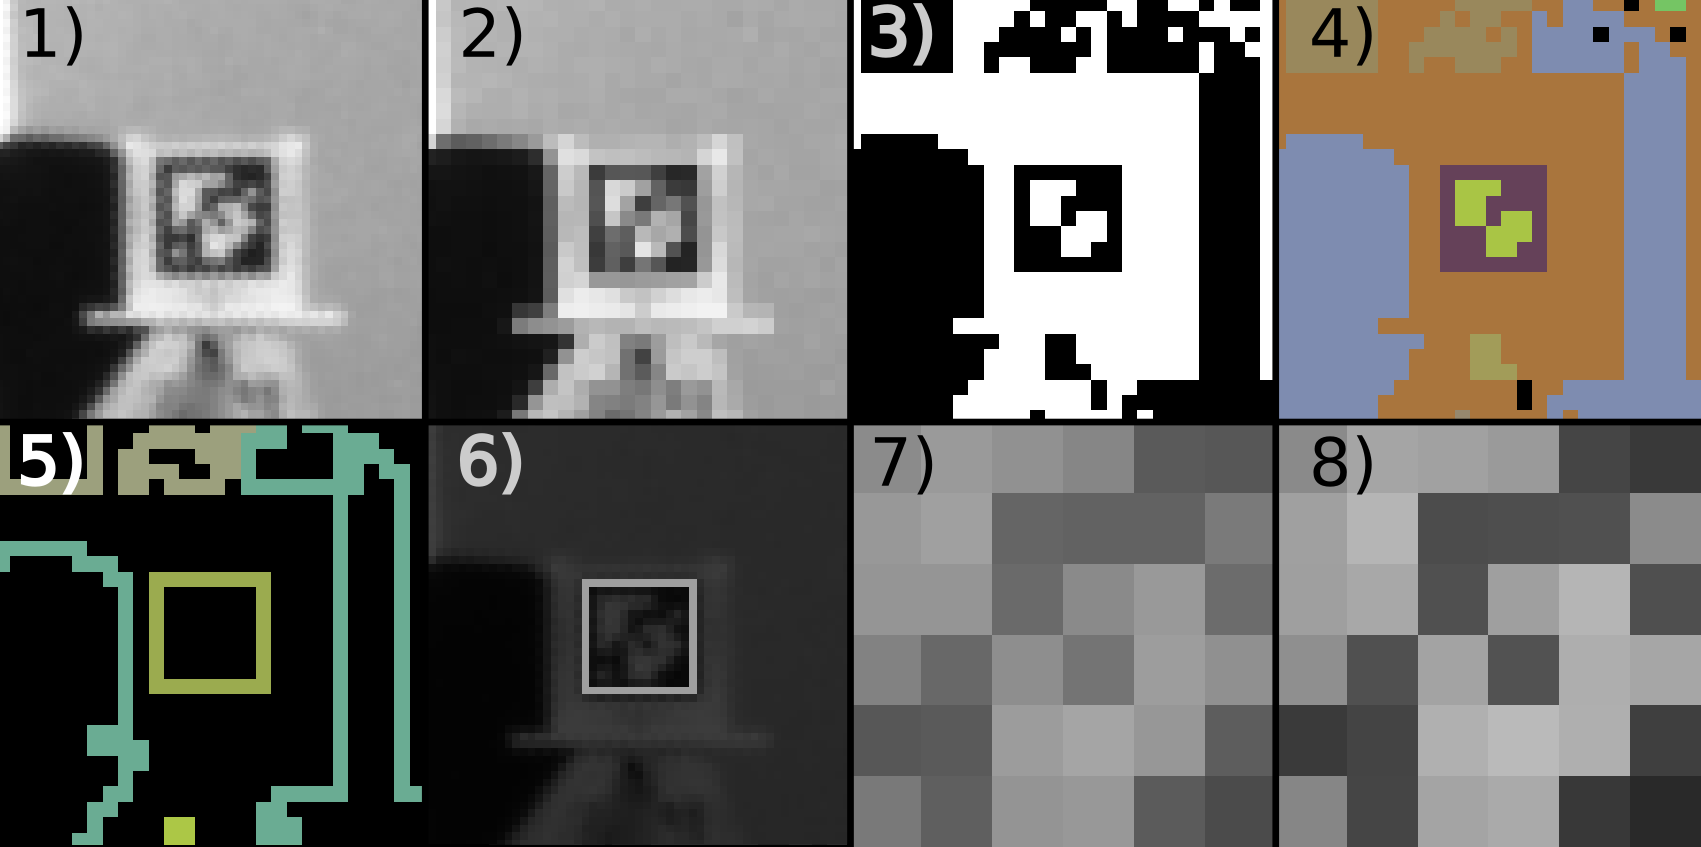
\includegraphics[width=0.9\textwidth]{img/detection/apriltag_alg.png}
  \caption[Postup při detekci AprilTagů]{Postup při detekci AprilTagů. 1) je vstup, 2) je vstup po decimaci, 3) prahování, 4) union-find, 5) segmentace souvislých hranic, 6) aproximace čtyřúhelníků z~hranic, 7) vyrovnání, 8) zvýšení ostrosti a dekódování. Převzato z~\cite{apriltag3}.}
  \label{fig:apriltagAlg}
\end{figure}

  \subparagraph{Adaptivní prahování} volí práh vždy lokálně v~závislosti na okolí prahovaného bodu jako aritmetický průměr minimálního a maximálního jasu. Pro snížení výpočetní náročnosti je v~tomto kroku vstupní obraz navíc decimován tak, že se extrémy hledají vždy v~buňkách po 4x4 pixelech, ve verzi 2 \cite{apriltag2} se autoři chtějí vyhnout nespojitostem na hranicích buněk a tak používají extrémy z~osmiokolí (po buňkách). Ve verzi 3 zjistili, že je vhodnější decimaci oddělit od prahování a používají bodové převzorkování, které lépe zachová hrany v~obrazu, ale může vést na aliasing \cite{apriltag3}. Zachování hran je vhodné, protože se v~dalším kroku detekují. Málo kontrastní body, které vzejdou z~prahování se v~dalším zpracování neuvažují, čímž jsou další kroky zrychleny.

  \subparagraph{Segmentace souvislých hranic} probíhá tím způsobem, že se nejprve najdou hrany v~prahovaném obrazu, čili takové pixely, které sousedí s~pixelem opačné barvy, jež se následně slučují do hranic pomocí algoritmu union-find. Problém, kdy jsou dva velmi blízké tagy odděleny pouze tenkou linií bílých pixelů, který by při sloučení hranic znemožňoval detekovat oba tagy zároveň, je vyřešen tak, že bílé pixely mohou být součástí 2 hranic. Každé takto segmentované části hranice je přiřazeno unikátní číslo v~rámci obrázku (tzv. obarvení). \cite{apriltag2}
  
  Zrychlení segmentace ve verzi 3 je docíleno tím, že se v~implementaci algoritmu zbytečně nesjednocují již sjednocené části (ušetří se volání sjednocení), navíc se včasně zamítají příliš malé oblasti, které by nemohly vést na dekódovatelný tag. \cite{apriltag3}

  \subparagraph{Aproximace čtyřúhelníku} z každého sjednocení v~předchozím kroku je provedeno vhodným dělením množiny hraničních bodů do 4 skupin, které odpovídají jednotlivým stranám odhadovaného čtyřúhelníku. Hledání optimálního řešení je příliš výpočetně náročné, proto se postupuje tak, že se mezi body naleznou kandidáti na rohy a poté se projdou všechny jejich kombinace. Rohy se hledají tak, že se body nejprve seřadí podle úhlu průvodiče vedeného z~centroidu množiny a jednotlivými body, poté se postupně aproximují body v~posuvném okně přímkou a hledají se maxima střední kvadratické chyby (\acrshort{mse}), odpovídající body jsou prohlášeny za rohy. Pro každou podmnožinu 4 rohů se zbylé body rozdělí na strany a každá z~nich se aproximuje přímkou. Vybere se taková kombinace rohů, pro kterou je \acrshort{mse} nejnižší. \cite{apriltag2}
  
  Ve verzi 3 se řazení bodů provádí podle kvadrantu, ve kterém se bod nachází a sklonu průvodiče. Není tak nutné počítat explicitně úhel. \cite{apriltag3}

  \subparagraph{Rychlé dekódování} tagů v~nalezených čtyřúhelnících probíhá tak, že se nejprve vyrovnají (pomocí homografie vypočtené ze souřadnic polohy jejich rohů) a hledá se nejbližší kód z~dané rodiny značek pro každou ze 4 možných rotací. Omezí-li se počet odlišných bitů na 2, je možné předpočítat všechny tagy maximálně 2 bity vzdálené od validního tagu a zaznamenat je do hashovací tabulky. Při detekci se z~tabulky jen vybere příslušná hodnota, nebo se detekce zamítne. \cite{apriltag2}
  
  Verze 3 zavádí bilineární interpolaci buněk tagu a zvyšuje ostrost za účelem zlepšení detekce malých značek. \cite{apriltag3}